\section{Příklad 1}
% Jako parametr zadejte skupinu (A-H)
\prvniZadani{E}

\graphicspath{{fig/pr1/}}
\begin{figure}[H]
\centering

\caption{Pôvodný obvod}
\end{figure}
\bigskip
\centerline{\Large{Poďme zjednodušovať!}}
\begin{figure}[H]
\centering
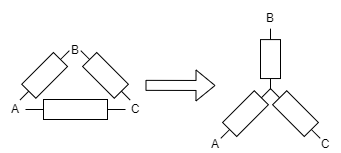
\includegraphics{hviezda.png}
\caption{Spravíme hviezdu}
\end{figure}
\begin{figure}[H]
\centering
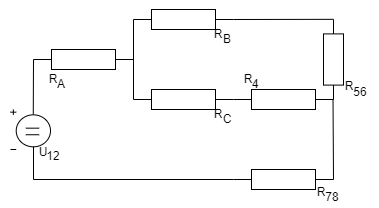
\includegraphics{uprava1.png}
\caption{Vymeníme $R_1, R_2, R_3$ za hviezdu a spojíme zdroje}
\end{figure}
\begin{figure}[H]
\centering
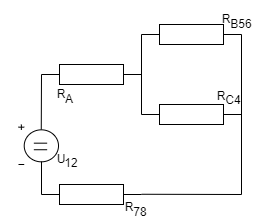
\includegraphics{uprava2.png}
\caption{Spájame rezistory}
\end{figure}
\begin{figure}[H]
\centering
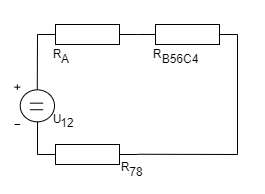
\includegraphics{uprava3.png}
\caption{Pokračujeme v ich spájaní}
\end{figure}
\begin{figure}[H]
\centering
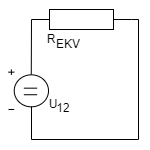
\includegraphics{uprava4.png}
\caption{A máme hotovo}
\end{figure}


\newpage

\centerline{\Large{Poďme rátať!}}
\centerline{Po úprave na hviezdu:}
\centering
\scalebox{1.5}{$U_{12} = U_1 + U_2\hspace{2em}$}
\scalebox{1.5}{$R_{56} = \frac{R_5 \times R_6}{R_5 + R_6}\hspace{2em}$}
\scalebox{1.5}{$R_A = \frac{R_1 \times R_2}{R_1 + R_2 + R_3}\hspace{2em}$}
\scalebox{1.5}{$R_B = \frac{R_1 \times R_3}{R_1 + R_2 + R_3}\hspace{2em}$}
\scalebox{1.5}{$R_C = \frac{R_2 \times R_3}{R_1 + R_2 + R_3}\hspace{2em}$}
\scalebox{1.5}{$R_{78} = R_7 + R_8$}
\\
\bigskip
\centerline{Po 1. spojení rezistorov (obrázok č. 4)}
\scalebox{1.5}{$ R_{B56} = R_B + R_{56} = \frac{R_1 \times R_3}{R_1 + R_2 + R_3} + \frac{R_5 \times R_6}{R_5 + R_6} $}\\
\bigskip
\scalebox{1.5}{$R_{C4} = R_C + R_4 = \frac{R_2 \times R_3}{R_1 + R_2 + R_3} + R_4$}\\
\bigskip
\centerline{Po 2. spojení rezistorov (obrázok č. 5)}
\scalebox{1.5}{$ R_{B56C4} = \frac{R_{B56} \times R_{C4}}{R_{B56} + R_{C4}} = \frac{(\frac{R_1 \times R_3}{R_1 + R_2 + R_3} + \frac{R_5 \times R_6}{R_5 + R_6}) \times (\frac{R_2 \times R_3}{R_1 + R_2 + R_3} + R_4)}{ (\frac{R_1 \times R_3}{R_1 + R_2 + R_3} + \frac{R_5 \times R_6}{R_5 + R_6}) + (\frac{R_2 \times R_3}{R_1 + R_2 + R_3} + R_4)} $}\\
\bigskip
\centerline{Po získaní $R_{EKV}$ (obrázok č. 6)}
\scalebox{1.12}{$ R_{EKV} = R_{B56C4} + R_{78} + R_A = \frac{(\frac{R_1 \times R_3}{R_1 + R_2 + R_3} + \frac{R_5 \times R_6}{R_5 + R_6}) \times (\frac{R_2 \times R_3}{R_1 + R_2 + R_3} + R_4)}{ (\frac{R_1 \times R_3}{R_1 + R_2 + R_3} + \frac{R_5 \times R_6}{R_5 + R_6}) + (\frac{R_2 \times R_3}{R_1 + R_2 + R_3} + R_4)} + R_7 + R_8 + \frac{R_1 \times R_2}{R_1 + R_2 + R_3} $}\\
\bigskip
\centerline{\Large{Postupne dosadíme a vyrátame $I_{R2}$ a $U_{R2}$!}}
\bigskip
\scalebox{1.5}{$ U_{12} = 115 + 55 = 170V $}\\
\bigskip
\scalebox{1.14}{$ R_{EKV} = \frac{(\frac{485 \times 100}{485 + 660 + 100} + \frac{575 \times 815}{575 + 815}) \times (\frac{660 \times 100}{485 + 660 + 100} + 340)}{(\frac{485 \times 100}{485 + 660 + 100} + \frac{575 \times 815}{575 + 815}) + (\frac{660 \times 100}{485 + 660 + 100} + 340)} + 255 + 225 + \frac{485 \times 660}{485 + 660 + 100} = \frac{\num{820 238 487 880}}{\num{882 847 843}}\Omega $}\\
\bigskip
\scalebox{1.5}{$ I=\frac{U_{12}}{R_{EKV}} = \frac{170}{\frac{\num{820 238 487 880}}{\num{882 847 843}}} = \frac{\num{15 008 413 331}}{\num{82 023 848 788}}A $}\\
\bigskip
\scalebox{1.5}{$ U_{R_A} = R_{A} \times I = \frac{485 \times 660}{485 + 660 + 100} \times \frac{\num{15 008 413 331}}{\num{82 023 848 788}} = \frac{\num{964 697 411 095}}{\num{20 505 962 197}}V $}\\
\bigskip
\scalebox{1.09}{$ U_{R_{B56C4}} = R_{B56C4} \times I = \frac{(\frac{485 \times 100}{485 + 660 + 100} + \frac{575 \times 815}{575 + 815}) \times (\frac{660 \times 100}{485 + 660 + 100} + 340)}{(\frac{485 \times 100}{485 + 660 + 100} + \frac{575 \times 815}{575 + 815}) + (\frac{660 \times 100}{485 + 660 + 100} + 340)} \times \frac{\num{15 008 413 331}}{\num{82 023 848 788}} = \frac{\num{102 900 937 525}}{\num{2 929 423 171}}V $}\\
\bigskip
\scalebox{1.5}{$ I_{R_{C4}} = \frac{U_{R_{B56C4}}}{R_{B56}} = \frac{\frac{\num{102 900 937 525}}{\num{2 929 423 171}}}{\frac{660 \times 100}{485 + 660 + 100} + 340} = \frac{\num{7 331 139 755}}{\num{82 023 848 788}}A $}\\
\bigskip
\scalebox{1.5}{$ U_{R_C} = I_{R_{C4}} \times R_C = \frac{\num{7 331 139 755}}{\num{82 023 848 788}} \times \frac{660 \times 100}{485 + 660 + 100} = \frac{\num{8 064 253 730 500}}{\num{2 112 114 106 291}}V $}\\
\bigskip
\scalebox{1.23}{$ U_{R_2} = U_{R_A} + U_{R_C} = \frac{\num{964 697 411 095}}{\num{20 505 962 197}} + \frac{\num{8 064 253 730 500}}{\num{2 112 114 106 291}} = \frac{\num{107 428 087 073 285}}{\num{2 112 114 106 291}}V \approx \underline{\underline{50.8628V}} $}\\
\bigskip
\scalebox{1.5}{$ I_{R_2} = \frac{U_{R_2}}{R_2} = \frac{\frac{\num{107 428 087 073 285}}{\num{2 112 114 106 291}}}{660} = \frac{\num{1 953 237 946 789}}{\num{25 345 369 275 492}}A \approx \underline{\underline{0.0771A}} $}









